\documentclass[../main.tex]{subfiles}
%!TEX root = ./analysisSnapFit.tex
\graphicspath {{../}}

\begin{document}
\subsection{Bearing Mounting (Snap-Fit)} \label{snapFit}
\begin{figure}[H]
	\centering
	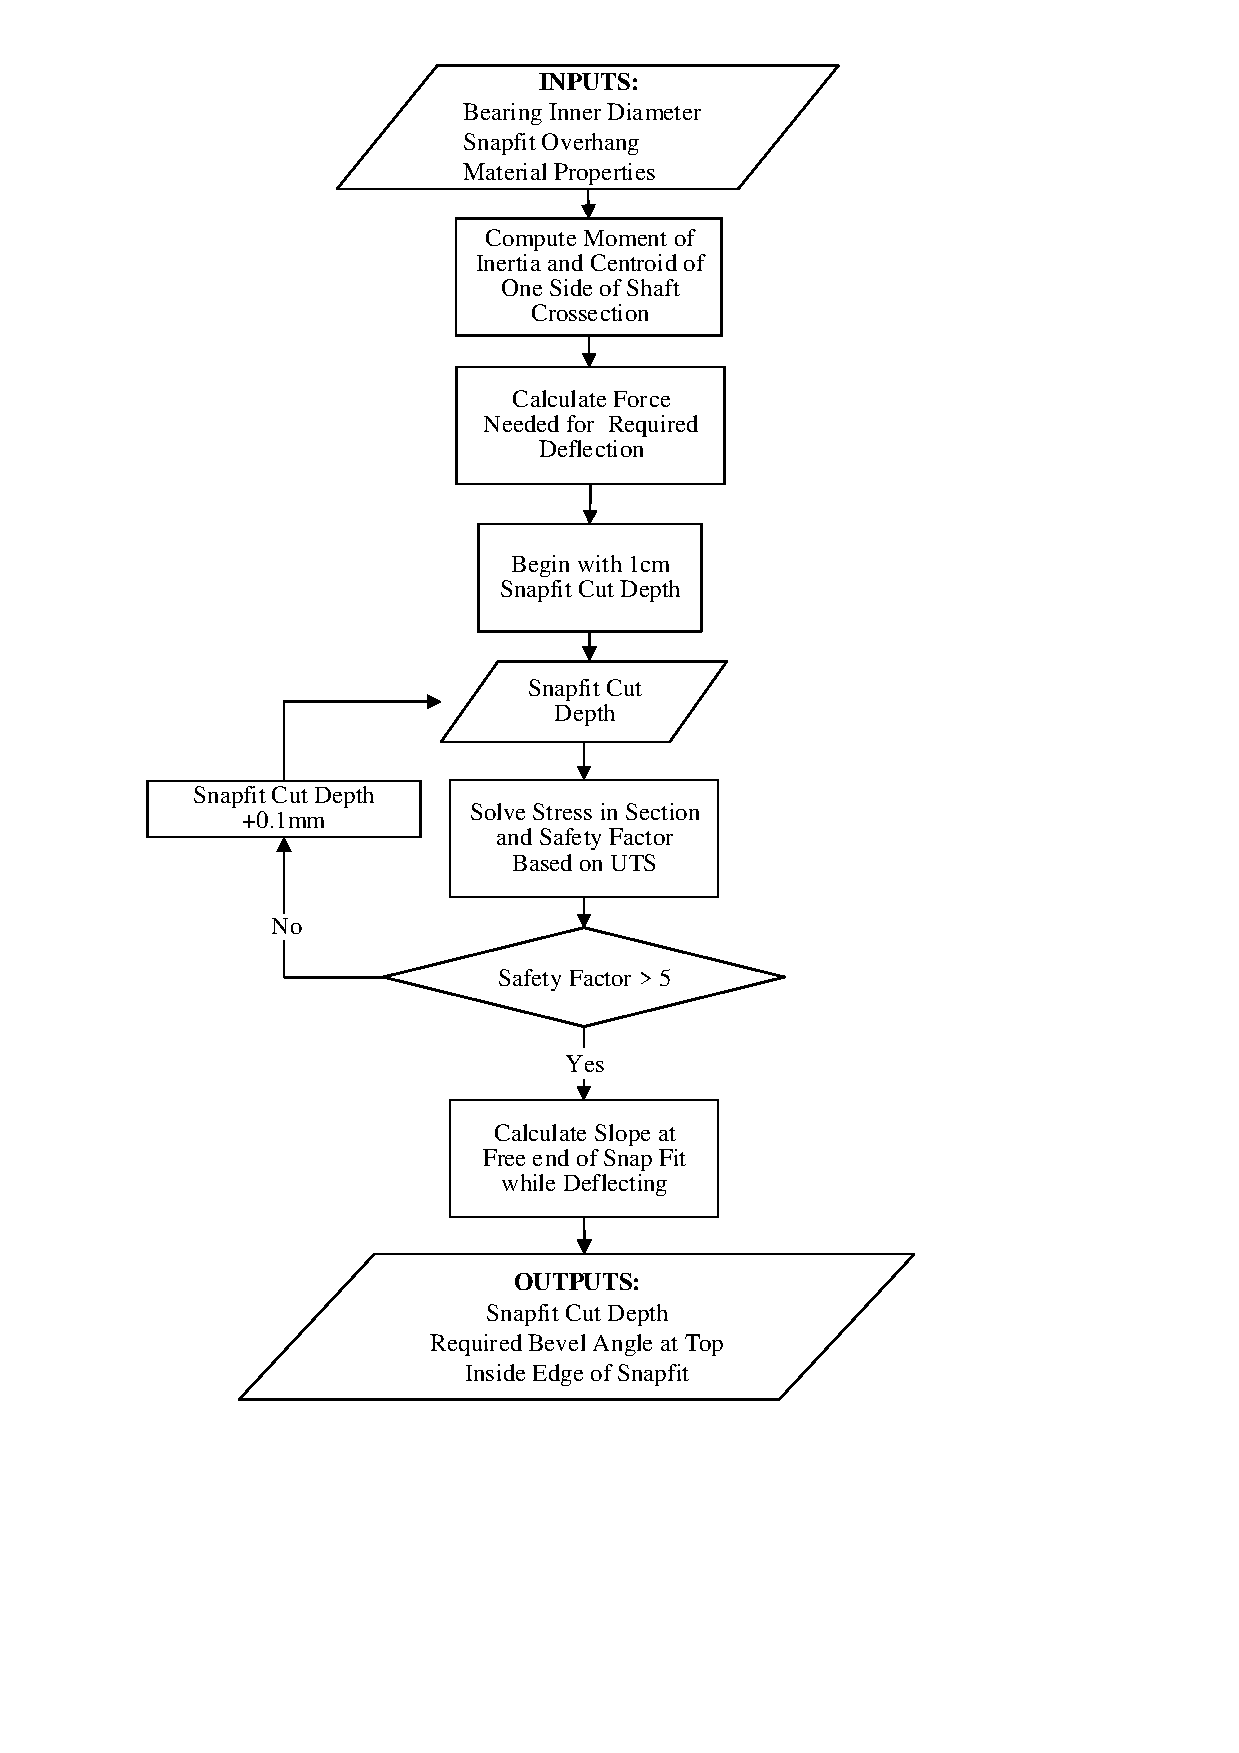
\includegraphics[width=0.82 \textwidth]{img/Paramaterization/snapFit.pdf}
	\caption{Parametrization Outline of Snapfit Analysis}
	\label{fig:snapParamaterization}
\end{figure}

The snapfit piece will be subject to a high load when the bearing is being installed, as significant deflection is necessary to allow the bearing into the grooved area. To account for this, there is a gaped section between the arms that allow for deflection. The bearing snap fit will be subject to potential failure at point at the outer edge of the shaft at the bottom of the snap fit cut shown in Figure \ref{Snapfit}. The analysis determines the minimum required cut depth in order to meet a safety factor of 1.5 as well as the bevel angle $\vartheta_{snap}$. the require inputs for this analysis are the bearing shaft diameter, the snap fit overhang and the material properties of nylon 12. These values are both constant as the shaft diameter is based on the inner diameter of the bearing used which will not be changing, this is justified by the analysis done in the Appendix Section \ref{gondolaBearings}. The choice of overhang coincides with the dimensions of the bearing used which can be seen in Appendix Datasheet \ref{PBearings}.

\begin{figure}[H]
	\centering
	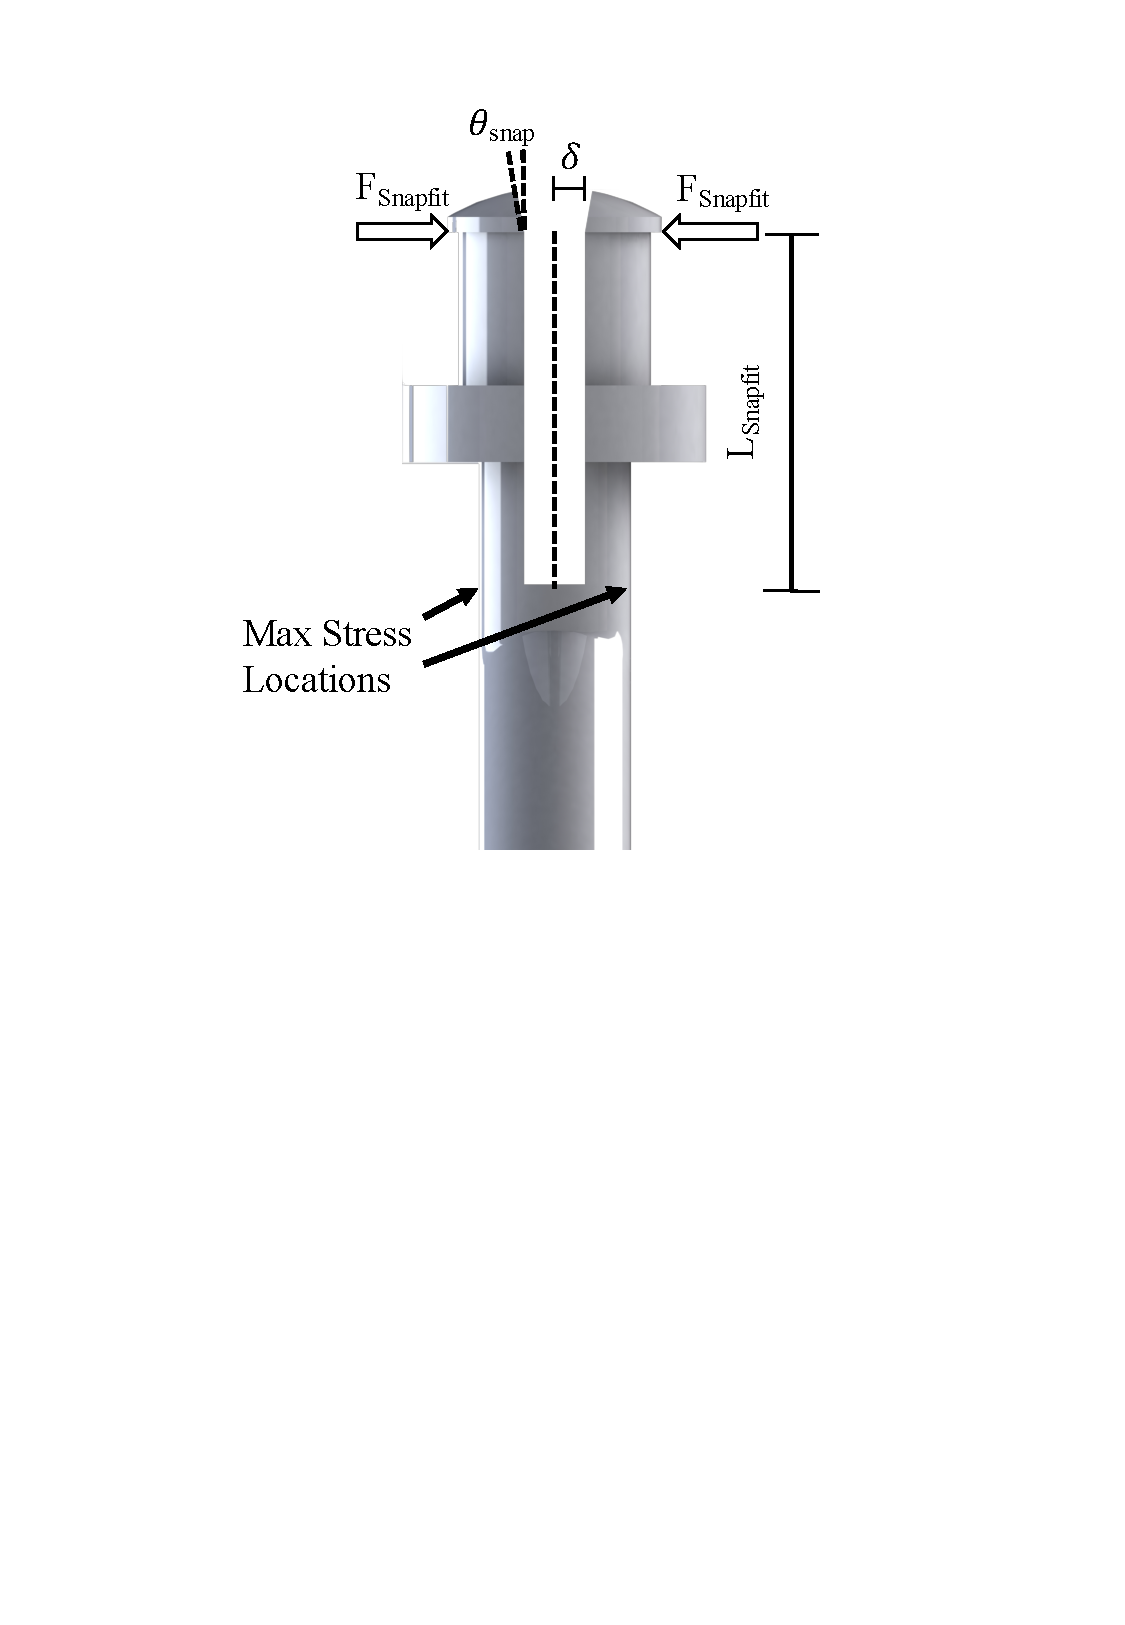
\includegraphics[width=1\textwidth]{img/gondola/Snapfit.pdf}
	\caption{Snapfit on Bearing Arm With Significant Dimensions }
	\label{fig:Snapfit}
\end{figure}

The analysis first computes the the force required for the deflection that must occur for the the snap fit to close to allow the bearing to slide onto the shaft. This calculation is done based on an initially chosen cut depth. The over hang is 1mm so the required deflection $\delta$ of each side of the snap cut is 1mm. The force required to achieve the the 1mm deflection $F_{Snapfit}$ is calculated by modeling the snap fit as a cantilever beam with a concentrated load, cantilevered at the depth of the cut into the shaft $L_{Snapfit}$. 

\begin{equation}
\label{eqn:Fsnap}
F_{Snapfit} = \frac{3 \delta E I}{L_{snapfit}^3}
\end{equation}

Because of the geometry each side of the snap fit, the moment of inertia was calculated using Equations \ref{eqn:Isnap}. $\theta$ in the equation is the angle that forms between the point in the center of the cut edge and the outside of the cut edge as seen in Figure \ref{fig:circleSection}.
\begin{figure}[H]
	\centering
	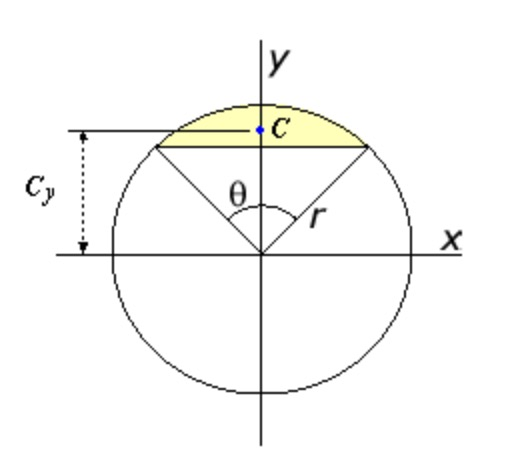
\includegraphics[width=0.6\textwidth]{img/Gondola/circleSectionGeometry.jpg}
	\caption{Centeroid of Section of Circle \cite{circlesection}}
	\label{fig:circleSection}
\end{figure}

\begin{equation}
\label{eqn:Isnap}
I = \left(\frac{r_{Snap}^4}{8}\right)  \left(\theta -\sin(\theta)+2\sin(\theta)(\sin^2\left(\frac{\theta}{2}\right))\right)
\end{equation}

The maximum stress $\sigma_{Snapfit}$ will occur at at the outer edge of the shaft at the bottom of the snap fit cut shown in Figure \ref{Snapfit}, and is calculated using the following equation.

\begin{equation}
\label{eqn:snapStress}
\sigma_{Snapfit} = \frac{F_{Snapfit} L_{snapfit} c}{I}
\end{equation}

The distance from the point the force is being applied to the neutral axis $c$ in equation \ref{eqn:snapStress}, is calculated by computing the length $C_y$ from Figure \ref{fig:circleSection} and subtracting it from the shaft radius plus the snap fit overhang. This can be seen in equation \ref{eqn:centroid}. 

 \begin{equation}
 \label{eqn:centroid}
 c = r_{overhang} - \frac{4r_{Snap}}{3}\left(\frac{\sin^3\left(\frac{\theta}{2}\right)} {\theta-\sin(\theta)}\right)
 \end{equation}

 This safety factor is slightly lower than other analysis with high failure likelihood which can be found in in table \ref{allComponents}. This is due to the fact that the installation will only be performed once. Maximum stress under normal loading conditions will be a direct result of the normal force applied on the bearing by the keel.


\end{document}